\chapter{Observing with small optical telescopes}

In this lab, we will be using a reflecting optical telescope to observe objects in the KPTC
lab. This will give you practice using the CCD camera to take images. More importantly,
these activities aim to give you a sense of scale for what the combined telescope and CCD are
capable of, and why this is useful for astronomical observations. The goal is for you to build some
understanding and appreciation for how telecopes of this size, equipped with a digitial camera and
filters, can be used to take images, and how those images relate to the capabilities of your most
familiar imaging system --- i.e. your eye.
%Your project work with the Stone Edge Observatory use a similar (although somewhat larger telescope) setup; this lab is designed to let you
%get your hands on the hardware and build some understanding for how it works and what it can
%do.

%\textbf{Rubric Rows to be assessed:} B5, B9, D2, D4. These are referenced in the lab manual where they should be addressed.

\section{Reflection Telescopes}

The primary utility of a telescope is its ability to gather light, thereby enabling visualization and analysis of the faint astronomical objects we are trying to observe. This requires focusing light incident on a large surface area. We will be using a \textbf{reflecting} telescope, which means that light rays from observation targets are focused into an eyepiece or onto a detector with reflecting mirrors. This is in contrast to refracting telescopes, which use refracting lenses to focus light rays. Figure~\ref{sot:fig:schmidt} shows schematically how this kind of telescope works. 

\begin{figure}
	\centering
	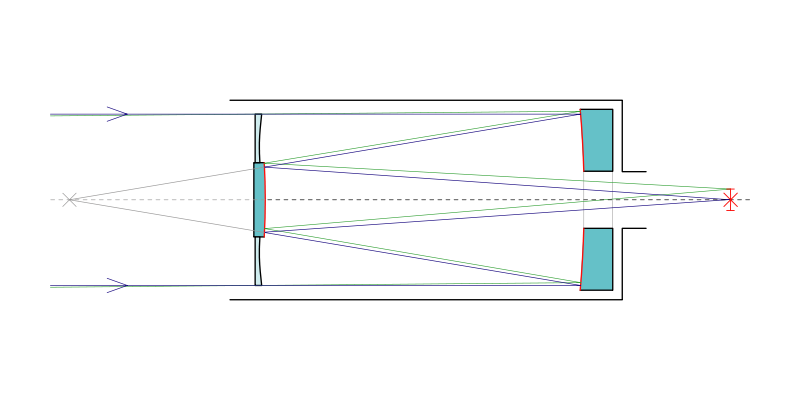
\includegraphics[scale = 0.5]{small-optical-telescopes/Schmidt-Cassegrain-Telescope.png}
	\caption{Schematic for a reflecting telescope of a Schmidt-Cassegrain design. 
		Light rays from astronomical objects enter the telescope in parallel because their source is effectively at infinity. They are then reflected by a parabolic primary mirror onto a secondary mirror that again reflects the light to a focus. An eyepiece or a camera is placed at the focal plane of the resulting image. Image source: \url{https://en.wikipedia.org/wiki/Cassegrain\_reflector\#/media/File:Schmidt-Cassegrain-Telescope.svg}}\label{sot:fig:schmidt}
\end{figure}

To take images in this lab,
% and to observe astronomical objects using the SEO,
 we make use of a \textbf{Charge Coupled Device (CCD)}. CCDs are the standard detectors for taking astronomical images at wavelengths blueward of approximately 1 micron. Think of the CCD we are using as a
very advanced low-noise digital detector, not wholly dissimilar from the digital detector in your
smartphone. Every time a photon within a certain energy range hits the detector, an electron is knocked off of the incident pixel, charging that pixel's capacitor. Thus, for each pixel, more photons $\implies$ more electrons $\implies$ more charge, and the charge can be read off into a digital signal that is then processed as an image. 

The main thing to note is that the CCD material is not sensitive to all wavelengths of light uniformly. Photons of certain energies are more likely to excite electrons in the detector and thus contribute to the output image. Consequently, the observed image intensity will be weighted by the response function of the detector.

\subsection{Filters}
Light is composed of photons with energies that determine their wavelengths (sorter wavelength $\implies$ higher energy). Thus every light source exhibits a textbf{spectrum} of energies based on its energetic components, determined by the physics of the light emission process. Thus, observing the energetic constituents of light from astronomical objects - a.k.a. observing the spectrum of emitted radiation - is a fundamental tool in observational astrophysics. However, obtaining the specific intensity of radiation as a function of energy from an astronomical source is challenging. An easier way to asses the electromagnetic energies observed is to image them in different filters: materials that are transparent to a known range of wavelengths and opaque to all others. Thus, one can image the same object with multiple different filters to get a sense of the wavelength regimes that make the strongest contributions to the overall electromagnetic output. 

A filter is characterized by its \textbf{transmission function}: a function that characterizes the amount of light that is transmitted by the filter at each wavelength. Figure~\ref{sot:fig:filters} shows the transmission functions for some standard astronomical filters (similar to the ones you'll be using in this class).

\begin{figure}
	\centering
	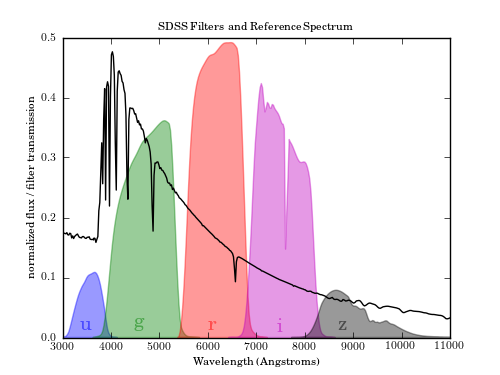
\includegraphics{small-optical-telescopes/fig_sdss_filters_1.png}
	\caption{Filter Transmission Functions for the Sloan Digital Sky Survey, overlaid on a stellar spectrum (in this case the spectrum is probably an
		A-type star). The magnitude observed by each filter will be proportional to the integrated spectrum multiplied by the filter transmission. It's clear in this image that the underlying spectrum of the star will cause the different filters to have different magnitudes. How would these magnitudes change if the spectrum was, say, of an M-star instead? (Image source: \url{http://www.astroml.org/\_images/fig\_sdss\_filters\_1.png})}\label{sot:fig:filters}
\end{figure}

\section{Lab Tasks: Introduction}

The telescope and camera assembly is an expensive and relatively fragile piece of hardware, so
move carefully when interacting with the system. We have only one setup, and there are
three main observing tasks, so before starting divide into three groups. Each group
will set up and control the telescope and camera for observing in one of the sections below, assisted by others in the lab, and
then share the output images with everyone in the lab group.

\section{Telescope Set Up, Preliminary ``Observations"}\label{sot:sec:setup}

First we will be observing an object at the opposite end of the lab room with the lights turned off. During this exercise we will 1) check that the telescope is focused (which should already be the case), 2) gain practice positioning the telescope and targets, and 3) demonstrate the light gathering and angular resolution capabilities of the telescope with a physical object for which you have an direct sense of scale. \textbf{NOTE: For safety purposes, do not walk around the
	lab while the lights are off; instead, turn the lights off only as needed to gather data
	or make observations, and when the lights are off, don’t move about significantly.}

\begin{steps}
	\item The telescope should already be set up, with the camera on and cooled, and be approximately
	in focus and pointed at the target at the other end of the lab bench. If not, your TA will
	work with you to get the setup roughly correct.
	
	\item Your first task will be to tweak the centering of the image target. This doesn't have to be
	perfect, but you should be able to see the mm scale marks. The telescope can be moved in elevation (up-down). The fine control of elevation is achieved using a knob on the mount - your TA will show you details. To shift the image left or right, move the target instead.
	
	\item Next we want to precisely focus the telescope. Do this with most of the lights off - otherwise
	the image has too much light. Use the 4th filter of the five available; this can be selected
	from the ‘Filter’ menu. Then, use the \textbf{Focus} task from the camera control system toolbar,
	and take images of a few seconds (at most). If the image is completely dark, and the peak intensity number in the focus box is reading around 65000, then the CCD is saturated, and the light in the room should be reduced, or the exposure time shortened.
	
	\item Start the focus sequence - the camera will just
	take and display images repeatedly, of the exposure duration you specified. Now, adjust
	the focus knob (on the back of the telescope, off center) until you achieve an optimal focus.
	Note that you can (and should) zoom the magnification of the image so you can see the
	imaging target in detail. Do this by adjusting the magnification, and adjusting the image
	x,y centering so you’re looking at an appropriate zoomed location in the image. Note that
	you’ll need to not be touching the telescope or mount to get a sharp image, so you’ll
	have to adjust, then move away, wait, and repeat. Your classmates walking around the lab
	will cause image shake that will make focusing difficult, so enforce a still classroom while
	you do this.
	
	\item Time to demonstrate one helpful aspect of telescopes by taking an image in the dark. Once the telescope is focused to the sharpest possible images, turn off the lights and acquire an image using the
	\textbf{Grab} button on the toolbar. An exposure time of 40--60 seconds is usually good with all of
	the lab lights off and the blinds closed.
	
	\item Save this image in ‘fits’ format; the ‘ds9’ tool available on all of the lab
	computers can be used to examine the image in detail.
%	We’ll use the university supported ’Box’ system to share data with your lab classmates.
%	See \url{uchicago.account.box.com/login} for details.
	
	\item With the lights back on, gather around the target on the lab bench and then
	turn the light off again. Observe the target. Can you see it? Can you see the details? Does
	it matter how close you are?% (Rubric Row B5)?
	
	\item Compute and report the ratio of the light gathering power of
	the telescope relative to your eye, and comment on how that relates to what you do (or do
	not) observe by eye compared to the telescope.% (Rubric Row B9).
	
	\item In the acquired and saved image you can see a mm scale, which correponds to some number
	of pixels. Compute and report the ‘plate scale’ in mm/pixel. Given the distance between the
	telescope and the target, what is the angular plate scale in arcseconds/pixel?
	
	To find this, note that for an arc (segment) of a circle, the length of that arc $s$ is related to the radius of circle $r$, and the angle (in radians) subtended by that arc $\theta$ by
	\begin{equation}
	 s = r \theta
	\end{equation}
	
	\item What do you
	think is the smallest feature (in arcsec) that you could resolve using this setup? Would we
	expect to see images of stars that sharp if we turned the telescope and camera skyward?
	Also, what is the field of view (arcseconds $\times$
	arcseconds) of this camera+telescope setup? Finally, observe the target from the vantage
	point of the telescope by eye. What detail can you see? How does that compare to what
	you can see with the telescope?
\end{steps}

\section{Grating Spectrum and Filters}\label{sot:sec:grating}

The next portion of the lab will involve observing a grating spectrum projected onto a blank white
target. We will use this to understand how the filters work. In addition, you will combine the
outputs of this and the third portion of the lab to unambiguously identify the 5 filters in the filter
wheel.
\begin{steps}
	\item Replace the reticle target and box with the blank white target mounted in a stand. Ensure
	the stand is placed so the target occupies the same plane as the reticle target did (otherwise,
	you’ll need to refocus the telescope; The paper has a pen mark on it - use this a reference if you do need to tweak the focus.). Next, place the light box with the attached diffraction
	grating on the same wooden stand using in the previous section, pointed toward the white target, and plug the light box in.
	This should generate a rainbow on the target screen. You may need to turn the lab lights
	off to see the rainbow easily. This rainbow is the spectrum of the incandescent lamp inside
	the light box.
	
	\item Once you’ve configured the setup, turn the lab lights off, and grab an exposure of 1 second
	in the 4th filter (if this section follows the above, that filter should already be selected).
	The bright band in the image should be positioned in the center of the image. If not, adjust
	the position of the spectrum by rotating the stand holding the lightbox+grating around the
	vertical axis to move spectrum slightly left or right on the screen. Adjust until the light band of the image is centered left/right. Also,
	to center vertically so that the light fully covers the image along the vertical axis, you may
 adjust the telescope elevation. To do these adjustments, you may find it easiest to put the camera
	in focus mode again. Centering vertically is less important - so long as a significant portion
	of the image contains light on the vertical axis there is no particular need to fine-tune the
	vertical alignment.
	
	\item Once you have the telescope aligned and focused on the reflected grating spectrum, grab an
	image of 1 second for each filter available in the CCD filter wheel. Save each image and note
	the differences. Comparing the different images, where are the bands located? How constant is the intensity of
	light across the band in the horizontal direction? How broad/narrow are the bands? What
	is the physical explanation for these observations (see also the end of the next section)?
\end{steps}

\section{Indirect H-lamp observations}\label{sot:sec:h-lamp}

\begin{steps}
	\item Now we will make some observations to demonstrate the utility of the narrow-band filters.
	Turn off the lamp with the grating attached and remove it from the lab bench. Remove the
	white screen that was used to reflect the grating spectrum, and again place the reticle target
	on the box (same as the activities for Section~\ref{sot:sec:setup}) at that location and refocus on the target if necessary.
	
	\item If the Hydrogen lamp is not already in place and set up, place the Hydrogen lamp in front
	off to side, plug the tube of Hydrogen gas into the lamp stand, and plug this
	into an electrical outlet. Use the pedal to turn it on and make sure it’s working: it will be
	a bright and somewhat odd (to your eye) magenta color (why?). Also, have a look at the
	Hydrogen lamp by eye, using the unmounted gratings --- note what you see, and explain what you
	see in your lab report. How many emission lines are visible?
	
	\item Make sure the reticle target is in the field of view of the telescope, similar to Part 1. Turn
	off the lab room lights, leave the Hydrogen lamp off, and grab a 10 second image in each of
	the 5 filters. Save each image as a fits file, with a name that indicates the filter and lamp
	condition (for example ’\texttt{filter1nolight.fits}’ etc.) The image should be dark but the target should
	be visible at least in some cases. Now, turn on the Hydrogen lamp using the small attached
	pedal, and grab another set of images (one per filter, ten seconds in each case) and similarly
	save them. You may find it easier to take each filter sequentially, turning the lamp on and
	off, rather than doing all filters lamp off and then lamp on. Do what works best for you.
	
	\item One of the two narrowband filters in the wheel - see Figure~\ref{sot:fig:filters} to know
	which filters are narrow in wavelength - is an H-alpha filter that isolates emission at the
	wavelength of the H-alpha Balmer line. Which filter is this? Filter1? Filter2? Filter3?
	Explain, using the data taken.
\end{steps}

The filter wheel contains two narrow band and three broad band filters. As already indicated
above, one of the narrow band filters is H-alpha, and the other is OIII-5007 (an emission line
at 500.7nm from star forming regions that is strong in star-forming galaxies, such as the Milky
Way). The broad band filters are the g-band (’g’=green) r-band (’r’=red) i-band (’i’=infrared) ;
see Figure 2 for details.

\begin{steps}
	
	\item Based on the data taken in Sections~\ref{sot:sec:grating} and \ref{sot:sec:h-lamp}, deduce the identification of each filter; provide your final list in your lab report - i.e. filter 1 as ’this’, filter 2 is ’that’ etc. Describe step-by-step how you solved this problem.
% (Rubric Rows D2, D4 (do not worry about experimental uncertainties, since this is a qualitative problem)).
\end{steps}

\section{Optional Section: See yourself with a telescope!}

Time permitting, you can also take images of yourself with the telescope.
Try placing your hand where the imaging target are (use the wooden box a
rest stand). Take images at different wavelengths (if you stayed carefully
still, you could make a color composite), or even see what your fingers
look like in H-alpha light). Or, place a stool nearby, take a seat, and
snap a partial portrait. Your face is far too large to fit in the field of
view at that distance, but your eye would fit! (refocusing will be
necessary in this case...)

\section{Report checklist and grading}

Each item below is worth 10 points, and there is an additional 10 points for attendance and participation. See Appendix\ \ref{cha:lab-report-format} for guidance on writing the report and formatting tables and graphs.

\begin{itemize}
	
	\item Image of the target that you captured and qualitative observations (Steps 6--7)
	
	\item Ratio of light-gathering power (Step 8) with comments.
	
	\item Calculation of pixel scale, questions regarding resolution and field of view. (Steps 9--10)
	
	\item Images of spectrum with each filter with analysis (Step 13).
	
	\item Qualitative observations of the hydrogen emission with diffraction gratings (Step 15).
	
	\item Images of hydrogen emission with each filter and identification of H-alpha filter (Steps 16--17).
	
	\item Identification of each filter in the filter wheel, with justification (Step 18).
	
\end{itemize}